\chapter{关联矩阵}
\label{chap:graph-incidence-matrix}

四个测点分别记录了温度$3,2,1,0$。相连的两个测点温差有多大？如果换一种数据——把各管道的流量摆在边上——每个测点进出了多少流量？

这两个问题都从同一个地方开始：查找每条边的两个端点。把端点信息写进一张矩阵，就能把"沿边取差"和"按顶点汇总"统一起来。本章用同一张关联矩阵连接顶点函数和边函数，先在四点图上逐项演示，再推导一般结果。

两种计算的输入和输出恰好相反。给定顶点读数时，每条边得到一个差值；给定边上的流量时，每个顶点得到一个净流出量。进出恰好相抵的边流量构成环空间，能由顶点差分产生的边向量构成割空间。这两类空间正交互补，用生成树的边和树外的边可以各找一组基。

本章最后考察关联矩阵的方子式。带符号矩阵在一端记流出、另一端记流入，无符号矩阵在两个端点各计一次。这两种记账方式分别决定了什么时候方子式只能取$0$和$\pm1$。由此得到一条有用的结论：最大流和二部匹配的整数规划，在允许变量取分数值之后仍然存在整数最优解。

\section{图上的函数}
\label{sec:graph-vertex-edge-functions}

在同一张图上，我们可以给每个测点记录一个温度，也可以给每条管道记录一个流量。前一类数值附着在顶点上，后一类数值附着在边上。固定顶点与边的编号顺序后，这两组数各自排成列向量，构成顶点空间与边空间；关联矩阵正是连接这两个空间的线性算子。本节先建立顶点函数与边流量向量的坐标表示，再定义关联矩阵并完整推导它的两种作用。

\subsection{顶点函数}
\label{sec:incidence-vertex-functions}

图~\ref{fig:incidence-running-example}画出了本章反复使用的四点五边图$\mathcal{G}=(V,E)$。四条外圈边围成一个四元环，另有一条对角边连接顶点$1$和$3$。顶点集和边集分别为
\[
V=\{1,2,3,4\},\qquad E=\{12,23,34,41,13\},
\]
其中$ij$简记连接顶点$i$与$j$的边。图中每个顶点旁标注了一个实数读数，依次为$3,2,1,0$。

给每个顶点赋一个实数，就得到图上的一个\term{顶点函数}（vertex function）$f\colon V\to\mathbb{R}$。图的顶点与边决定哪些位置直接相连，函数值则是在这一连接结构上附加的观测或状态数据。同一张图在不同应用场景中可以承载测点温度、地面海拔或节点电势——底层的图结构不变，改变的只是顶点上的函数值。

\begin{figure}[!htb]
  \centering
  \begingroup
\definecolor{IncidenceBlue}{HTML}{7188A3}
\definecolor{IncidenceInk}{HTML}{3B4252}
\begin{tikzpicture}[
  x=2.55cm,y=1.68cm,
  incidence vertex/.style={circle,draw=FigureStroke,fill=white,
    line width=.68pt,minimum size=5mm,inner sep=0pt,
    font=\footnotesize,text=IncidenceInk},
  incidence edge/.style={-{Stealth[length=2mm]},draw=FigureStroke,line width=.82pt},
  incidence reading/.style={text=IncidenceInk,font=\footnotesize,inner sep=3pt}
]
  \node[incidence vertex] (one) at (0,1) {$1$};
  \node[incidence vertex] (two) at (1,1) {$2$};
  \node[incidence vertex] (three) at (1,0) {$3$};
  \node[incidence vertex] (four) at (0,0) {$4$};
  \draw[incidence edge] (one) -- (two);
  \draw[incidence edge] (two) -- (three);
  \draw[incidence edge] (three) -- (four);
  \draw[incidence edge] (four) -- (one);
  \draw[incidence edge,draw=IncidenceBlue] (one) -- (three);
  \node[incidence reading,left=3mm of one] {$f(1)=3$};
  \node[incidence reading,right=3mm of two] {$f(2)=2$};
  \node[incidence reading,right=3mm of three] {$f(3)=1$};
  \node[incidence reading,left=3mm of four] {$f(4)=0$};
\end{tikzpicture}
\endgroup

  \caption{本章的四点五边图及一组顶点读数。黑灰色实线是四条外圈环边，蓝色实线是对角边$13$。边上的箭头给出记录沿边差分与边流量时使用的参考方向。顶点旁标注的读数排成列向量$\bm{f}=(3,2,1,0)^\top$。}
  \label{fig:incidence-running-example}
\end{figure}

对$n=|V|$个顶点固定一个排列次序$v_1,\ldots,v_n$，把各点上的函数值按此顺序排成列向量，顶点函数$f$就与$n$维列向量
\[
\bm{f}=\bigl(f(v_1),\ldots,f(v_n)\bigr)^\top\in\mathbb{R}^n
\]
一一对应。两个顶点函数可以逐顶点相加，也可以同乘一个实数，运算规则与$\mathbb{R}^n$中的向量加法和数乘完全一致。因此，图上全体实值顶点函数构成一个$n$维线性空间，记为$\mathbb{R}^V\cong\mathbb{R}^n$。对每个顶点$v\in V$，仅在顶点$v$处取$1$、在其余顶点处均取$0$的单位脉冲函数对应标准基向量$\bm{e}_v\in\mathbb{R}^V$，全部$n$个顶点的标准基向量$\{\bm{e}_{v_1},\ldots,\bm{e}_{v_n}\}$构成$\mathbb{R}^V$的一组标准正交基，任意顶点函数均可展开为$\bm{f}=\sum_{v\in V}f(v)\bm{e}_v$。

在顶点空间$\mathbb{R}^V$上，两个顶点函数$\bm{f},\bm{g}$的标准内积定义为各顶点读数乘积之和：
\begin{equation}
\langle\bm{f},\bm{g}\rangle_V=\bm{f}^\top\bm{g}=\sum_{v\in V}f(v)\,g(v).
\label{eq:incidence-vertex-inner-product}
\end{equation}
有限维线性空间中的基、坐标与内积可参考\BookChapterRef{chap:linear-representation}{卷二"线性空间"章}。

重新给顶点编号相当于对向量坐标施加一次置换。例如将顶点排列次序从$1,2,3,4$改为$3,1,4,2$，列向量的四个分量随之重排，但每个测点本身的读数并未改变。只要在计算前固定一套顶点编号次序，向量的每个分量就唯一对应一个顶点。本章固定按$1,2,3,4$排列图~\ref{fig:incidence-running-example}中的读数，得到
\[
\bm{f}=(3,2,1,0)^\top.
\]
这组顶点读数将在后续计算中反复使用。

\subsection{边函数}
\label{sec:incidence-edge-functions}

与给每个顶点赋值的顶点函数相对应，给每条边赋一个实数就得到图上的一个\term{边函数}（edge function）$q\colon E\to\mathbb{R}$。对$m=|E|$条边固定一个编号次序$e_1,\ldots,e_m$，边函数$q$便与$m$维列向量
\[
\bm{q}=\bigl(q(e_1),\ldots,q(e_m)\bigr)^\top\in\mathbb{R}^m
\]
一一对应，全体实值边函数构成$m$维线性空间$\mathbb{R}^E\cong\mathbb{R}^m$。在图~\ref{fig:incidence-running-example}的四点五边图上，$m=5$；本章固定边的排列顺序为$12,23,34,41,13$，每个边函数写成五维列向量$\bm{q}=(q_{12},q_{23},q_{34},q_{41},q_{13})^\top\in\mathbb{R}^5$。

与顶点上的标量读数不同，沿边传递的量（如流量、电流或电位差）带有方向性。为了用实数坐标无歧义地记录方向，我们为每条无向边$e=\{u,v\}$预先指定一个箭头方向$u\to v$作为\emph{参考方向}（reference orientation），称$u$为该参考方向下的尾端（tail）、$v$为头端（head）。在图~\ref{fig:incidence-running-example}中，五条边的参考方向依次约定为$1\to2$、$2\to3$、$3\to4$、$4\to1$和$1\to3$。

当边函数用于记录沿边输送的有向数量时，在给定参考方向下，边空间中的向量$\bm{q}\in\mathbb{R}^E$称为图上的一个\term{边流量}（edge flow，也称边流量向量），其第$e$个分量$q_e\in\mathbb{R}$表示边$e$上的有向流量：
\begin{itemize}
\item 若$q_e>0$，表示边$e$上的实际流向与参考方向$u\to v$一致，流量大小为$q_e$；
\item 若$q_e<0$，表示边$e$上的实际流向与参考方向相反（即沿$v\to u$流动），流量大小为$|q_e|$；
\item 若$q_e=0$，表示边$e$上没有流量。
\end{itemize}
例如在边$41$（参考方向为$4\to1$）上，若记录$q_{41}=-2$，实际含义是从顶点$1$流向顶点$4$的流量为$2$个单位。对无向图而言，参考方向只是一种坐标记账约定：同一股实际物理流如果改用相反的参考方向记录，其坐标分量$q_e$变号，但实际流向与流量大小丝毫不变。

在后续章节中，我们需要严格区分边流量$q_e$与边权$w_e$这两类边上数据。边流量$\bm{q}\in\mathbb{R}^E$是随外部输入或状态变化的变量，反转边$e$的参考方向会使坐标$q_e$变号；而边权$w_e\geq 0$是图本身的结构参数（如管道容导、支路电导或连接强度），反转参考方向不会改变非负边权$w_e$的数值。后续将$m$条边的权重排成$m\times m$对角矩阵$\bm{C}=\operatorname{diag}(w_{e_1},\ldots,w_{e_m})$。

在边空间$\mathbb{R}^E$上，两个边向量$\bm{q},\bm{r}\in\mathbb{R}^E$的标准内积定义为对应边分量乘积之和：
\begin{equation}
\langle\bm{q},\bm{r}\rangle_E=\bm{q}^\top\bm{r}=\sum_{e\in E}q_e\,r_e.
\label{eq:incidence-edge-inner-product}
\end{equation}
本章讨论环空间与割空间的正交分解时始终使用这一标准内积。到第~\ref{chap:graph-electrical-networks}章研究电网络时，为了按支路电阻计量电功率耗散，还会引入以电阻矩阵加权的边内积；不同内积定义了不同的正交关系，使用时须加以区分。

\subsection{关联矩阵的作用}
\label{sec:incidence-matrix-actions}

建立了顶点空间$\mathbb{R}^V$和边空间$\mathbb{R}^E$之后，我们用一张矩阵把这两个空间连接起来。

给定有$n$个顶点、$m$条边的图$\mathcal{G}=(V,E)$并固定各边的参考方向。对每一条有向参考边$e\colon u\to v$，我们在矩阵的第$e$列中，于尾端$u$所在的行填$+1$，于头端$v$所在的行填$-1$，其余各行均填$0$。这样构造出的$n\times m$矩阵$\bm{B}\in\mathbb{R}^{n\times m}$称为图$\mathcal{G}$的\term{关联矩阵}（incidence matrix，更确切地称为带符号关联矩阵），其第$e$列可写为顶点空间两个标准基向量之差：
\begin{equation}
\bm{B}_{:,e}=\bm{e}_u-\bm{e}_v,\qquad e\colon u\to v.
\label{eq:incidence-oriented-column}
\end{equation}
由于无自环图的每条边连接两个不同端点，$\bm{B}$的每一列恰好含有一个$+1$和一个$-1$，其余$n-2$个元素全为$0$，因此每一列的元素之和恒等于零。

按顶点顺序$1,2,3,4$排矩阵的行，按边顺序$12,23,34,41,13$（参考方向依次为$1\to2,2\to3,3\to4,4\to1,1\to3$）排矩阵的列，图~\ref{fig:incidence-running-example}中四点五边图的关联矩阵为
\[
\bm{B}=
\begin{pmatrix}
 1 & 0 & 0 & -1 & 1\\
 -1 & 1 & 0 & 0 & 0\\
 0 & -1 & 1 & 0 & -1\\
 0 & 0 & -1 & 1 & 0
\end{pmatrix}.
\]
以第四列（对应边$41\colon 4\to1$）为例：尾端是顶点$4$，所以第$4$行填$+1$；头端是顶点$1$，所以第$1$行填$-1$；顶点$2$和$3$不是边$41$的端点，第$2,3$行均填$0$。

关联矩阵$\bm{B}$及其转置$\bm{B}^\top$分别诱导了方向相反的两个基本线性映射：$\bm{B}^\top\colon\mathbb{R}^V\to\mathbb{R}^E$把顶点函数映射为边空间中的向量，$\bm{B}\colon\mathbb{R}^E\to\mathbb{R}^V$把边流量向量映射回顶点空间。下面依次考察这两个映射的具体含义。

\paragraph{沿边取差}

先看转置矩阵$\bm{B}^\top\in\mathbb{R}^{m\times n}$对顶点函数$\bm{f}\in\mathbb{R}^V$的作用。$\bm{B}^\top$的第$e$行正是$\bm{B}$的第$e$列转置$(\bm{e}_u-\bm{e}_v)^\top$。用这一行左乘列向量$\bm{f}$，得到的第$e$个分量恰好是边$e\colon u\to v$的尾端读数$f(u)$减去头端读数$f(v)$：
\[
(\bm{B}^\top\bm{f})_e=(\bm{e}_u-\bm{e}_v)^\top\bm{f}=f(u)-f(v).
\]
对全部$m$条边同时执行这一运算，就得到边空间中的一个$m$维列向量$\bm{d}=\bm{B}^\top\bm{f}\in\mathbb{R}^E$，其第$e$个分量为
\begin{equation}
d_e=(\bm{B}^\top\bm{f})_e=f(u)-f(v),\qquad e\colon u\to v.
\label{eq:incidence-edge-difference}
\end{equation}
我们把由顶点函数$\bm{f}$生成的边向量$\bm{d}=\bm{B}^\top\bm{f}\in\mathbb{R}^E$称为$\bm{f}$的\term{沿边差分}（edge difference，或沿边差分向量），而把线性算子$\bm{B}^\top\colon\mathbb{R}^V\to\mathbb{R}^E$称为沿边差分算子。需要明确的是：单个分量$d_e=f(u)-f(v)$是边$e$上的标量差值，而$\bm{B}^\top\bm{f}$则是将所有边上的差值按边序排列而成的$m$维边向量。

我们在四点五边图上对读数$\bm{f}=(3,2,1,0)^\top$逐边计算其沿边差分向量$\bm{B}^\top\bm{f}$：
\begin{itemize}
\item 边$12$（$1\to2$）：$d_{12}=f(1)-f(2)=3-2=1$；
\item 边$23$（$2\to3$）：$d_{23}=f(2)-f(3)=2-1=1$；
\item 边$34$（$3\to4$）：$d_{34}=f(3)-f(4)=1-0=1$；
\item 边$41$（$4\to1$）：$d_{41}=f(4)-f(1)=0-3=-3$；
\item 边$13$（$1\to3$）：$d_{13}=f(1)-f(3)=3-1=2$。
\end{itemize}
将五个分量按边序排成列向量，得到
\[
\bm{B}^\top\bm{f}=(1,1,1,-3,2)^\top\in\mathbb{R}^5.
\]

如果给每个顶点的读数同时加上同一个常数$c\in\mathbb{R}$，即把$\bm{f}$替换为$\bm{f}+c\bm{1}$，那么任意一条边$e\colon u\to v$上的差值变为
\[
\bigl(f(u)+c\bigr)-\bigl(f(v)+c\bigr)=f(u)-f(v),
\]
常数增量$c$在尾端与头端相减时完全抵消。特别地，若顶点函数在所有顶点上取同一个常数$c$（即常值向量$\bm{f}=c\bm{1}$），则它的沿边差分向量为零向量$\bm{B}^\top(c\bm{1})=\bm{0}$——各点读数毫无差别，沿边自然没有变化。

\paragraph{按顶点汇总}

再看关联矩阵本身$\bm{B}\colon\mathbb{R}^E\to\mathbb{R}^V$对边流量向量$\bm{q}\in\mathbb{R}^E$的作用。按行读取$\bm{B}$：在第$v$行中，所有以顶点$v$为尾端（从$v$出发）的边系数为$+1$，所有以顶点$v$为头端（进入$v$）的边系数为$-1$，不以$v$为端点的边系数为$0$。因此，用$\bm{B}$的第$v$行左乘边流量向量$\bm{q}$，就是把从顶点$v$流出的总流量减去流入顶点$v$的总流量，所得结果称为顶点$v$处的\term{净流出量}（net outflow）：
\begin{equation}
(\bm{B}\bm{q})_v=\sum_{e:\,v\text{ 是尾端}}q_e
              -\sum_{e:\,v\text{ 是头端}}q_e.
\label{eq:incidence-net-outflow}
\end{equation}
将全部$n$个顶点的净流出量排成列向量，就得到顶点空间中的\emph{净流出向量}$\bm{B}\bm{q}\in\mathbb{R}^V$。

以四点图中的顶点$1$为例。$\bm{B}$的第一行在边$12,41,13$处非零：边$12$（$1\to2$）和边$13$（$1\to3$）以顶点$1$为尾端，系数为$+1$；边$41$（$4\to1$）以顶点$1$为头端，系数为$-1$。因此顶点$1$的净流出量为
\[
(\bm{B}\bm{q})_1=q_{12}-q_{41}+q_{13}.
\]

为了看清单条边上的流量如何影响各个顶点，取只在第一条边$12$上携带$1$个单位正向流量的边流量向量$\bm{q}=\bm{e}_{12}=(1,0,0,0,0)^\top$。左乘$\bm{B}$恰好取出$\bm{B}$的第一列：
\[
\bm{B}(1,0,0,0,0)^\top=(1,-1,0,0)^\top.
\]
可以看到，尾端顶点$1$的净流出量为$+1$，头端顶点$2$的净流出量为$-1$（即净流入$1$），其余顶点$3,4$的净流出量均为$0$。

一般的边流量向量$\bm{q}=\sum_{e\in E}q_e\bm{e}_e$是各条边流量的叠加，对应的净流出向量为
\[
\bm{B}\bm{q}=\sum_{e\colon u\to v}q_e(\bm{e}_u-\bm{e}_v).
\]
在每一条边$e\colon u\to v$上，从尾端$u$流出的量$+q_e$必定等于进入头端$v$的量（记作净流出$-q_e$）。把所有$n$个顶点的净流出量相加，即用全一向量$\bm{1}^\top$左乘$\bm{B}\bm{q}$，每条边的$+q_e$与$-q_e$都成对抵消：
\[
\sum_{v\in V}(\bm{B}\bm{q})_v
=\bm{1}^\top(\bm{B}\bm{q})
=\sum_{e\colon u\to v}(q_e-q_e)=0.
\]
这说明：无论边流量向量$\bm{q}\in\mathbb{R}^E$取何值，全图所有顶点的净流出量总和恒为零。

图~\ref{fig:incidence-matrix-actions}把$\bm{B}^\top$与$\bm{B}$的两种基本计算放在同一条参考边$1\to2$上并排对照：左图由两端读数$f(1)=3,f(2)=2$相减得到该边上的沿边差分分量$d_{12}=1$；右图由该边上的单位流量$q_{12}=1$在尾端$1$记净流出$+1$、在头端$2$记净流出$-1$。

\begin{BookInlineFigure}
  \centering
  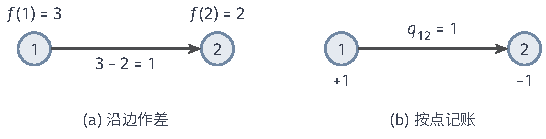
\includegraphics{figures/03-graphs/05-matrices-and-spectra/tikz/incidence-matrix-actions/figure.pdf}
  \caption{同一条参考边$1\to2$上的两种对偶运算。(a) 沿边差分算子$\bm{B}^\top$将两端顶点读数作差，得到边分量$d_{12}=f(1)-f(2)=1$。(b) 净流出汇总算子$\bm{B}$将该边上的单位正向流量$q_{12}=1$分配到两端，尾端净流出为$+1$，头端净流出为$-1$。}
  \label{fig:incidence-matrix-actions}
\end{BookInlineFigure}

\paragraph{伴随恒等式}

沿边差分算子$\bm{B}^\top\colon\mathbb{R}^V\to\mathbb{R}^E$与按顶点汇总算子$\bm{B}\colon\mathbb{R}^E\to\mathbb{R}^V$在矩阵形式上互为转置，在几何上则关于顶点内积与边内积互为伴随算子。

任取一个顶点函数$\bm{f}\in\mathbb{R}^V$和一个边流量向量$\bm{q}\in\mathbb{R}^E$。先算出沿边差分向量$\bm{B}^\top\bm{f}\in\mathbb{R}^E$，再与$\bm{q}$在边空间中作内积，按式~\eqref{eq:incidence-edge-inner-product}展开为对所有边的求和：
\[
\langle\bm{B}^\top\bm{f},\bm{q}\rangle_E
=\sum_{e\colon u\to v}\bigl(f(u)-f(v)\bigr)q_e
=\sum_{e\colon u\to v}\bigl(f(u)q_e-f(v)q_e\bigr).
\]
在最右端的求和式中，每条边$e\colon u\to v$产生了两项：尾端$u$处带有正号项$+f(u)q_e$，头端$v$处带有负号项$-f(v)q_e$。现在把求和次序从“逐边相加”改为“逐顶点归并”：固定一个顶点$w\in V$，把所有以$w$为尾端的边所贡献的$+f(w)q_e$与所有以$w$为头端的边所贡献的$-f(w)q_e$收集到一起，提出公因子$f(w)$，括号内剩下的恰好就是式~\eqref{eq:incidence-net-outflow}中顶点$w$的净流出量$(\bm{B}\bm{q})_w$：
\[
\begin{aligned}
\sum_{e\colon u\to v}\bigl(f(u)q_e-f(v)q_e\bigr)
&=\sum_{w\in V}f(w)\Biggl(\sum_{e:\,w\text{ 是尾端}}q_e-\sum_{e:\,w\text{ 是头端}}q_e\Biggr)\\
&=\sum_{w\in V}f(w)(\bm{B}\bm{q})_w.
\end{aligned}
\]
根据顶点内积定义式~\eqref{eq:incidence-vertex-inner-product}，最右端正是$\bm{f}$与净流出向量$\bm{B}\bm{q}$在顶点空间中的内积。于是我们得到伴随恒等式：
\begin{equation}
\langle\bm{B}^\top\bm{f},\bm{q}\rangle_E
=\langle\bm{f},\bm{B}\bm{q}\rangle_V.
\label{eq:incidence-adjoint-pairing}
\end{equation}
从代数上看，式~\eqref{eq:incidence-adjoint-pairing}就是向量内积的转置性质$(\bm{B}^\top\bm{f})^\top\bm{q}=\bm{f}^\top(\bm{B}\bm{q})$；从图上的记账来看，它表明“按每条边把两端读数差乘以边流量再求和”与“按每个顶点把读数乘以净流出量再求和”算的是同一笔总账。下一节证明环空间与割空间正交时，这一恒等式将起到核心作用。

最后说明参考方向的选择对计算结果的影响。如果将某一条边$e$的参考方向从$u\to v$反转为$v\to u$，矩阵$\bm{B}$的第$e$列随之变号；与此同时，同一股实际流量在新参考方向下的坐标$q_e$也变号。在计算$\bm{B}\bm{q}$时，列向量的负号与流量坐标的负号相乘抵消，因此每个顶点的净流出量$(\bm{B}\bm{q})_v$完全不变。

同理，沿边差分分量$(\bm{B}^\top\bm{f})_e$虽随参考方向变号，但与同样变号的$q_e$相乘后乘积不变。这意味着参考方向只是边空间坐标系的符号约定，顶点处的物理守恒关系以及下一节建立的子空间结构均不依赖于参考方向的具体选取。

\section{环空间与割空间}
\label{sec:graph-cycle-cut-spaces}

上一节建立了关联矩阵的两种对偶运算：沿边差分算子$\bm{B}^\top\colon\mathbb{R}^V\to\mathbb{R}^E$把顶点函数变成沿边差分向量，净流出汇总算子$\bm{B}\colon\mathbb{R}^E\to\mathbb{R}^V$把边流量向量变成各顶点的净流出量。这两个算子在边空间$\mathbb{R}^E$中自然划分出两类核心子空间——在所有顶点处净流出均为零的边流量构成环空间$\ker\bm{B}$，由顶点函数沿边差分生成的边向量构成割空间$\operatorname{im}\bm{B}^\top$。

本节依次建立这两个子空间的定义、正交直和分解与维数公式，最后利用生成森林构造出两组可直接读出坐标的显式基。

\subsection{环空间}
\label{sec:incidence-cycle-space}

我们先在图~\ref{fig:incidence-running-example}的四点五边图上考察什么样的边流量向量能使每个顶点的净流出量都等于零。

第一股流量沿外圈四元环$1\to2\to3\to4\to1$依次输送$1$个单位，对角边$13$上不送流。在每个顶点处核对进出账目：在顶点$1$，边$12$流出$1$个单位、边$41$流入$1$个单位，净流出为零；在顶点$2$，边$12$流入$1$个单位、边$23$流出$1$个单位，净流出也为零；顶点$3$与顶点$4$同理。因为外圈四条边的绕行方向与图~\ref{fig:incidence-running-example}约定的参考方向完全一致，按边序$(12,23,34,41,13)$记录，这股边流量向量为
\[
\bm{c}_1=(1,1,1,1,0)^\top.
\]
代入关联矩阵直接验算，确实有$\bm{B}\bm{c}_1=\bm{0}$。

第二股流量沿三角形回路$1\to3\to2\to1$绕行$1$个单位，外圈边$34$和$41$上不送流。逐边核对绕行方向与参考方向的关系：在对角边$13$上，绕行从$1$到$3$，与参考方向$1\to3$一致，分量取$+1$；在边$23$和边$12$上，绕行分别从$3$到$2$、从$2$到$1$，均与各自的参考方向（$2\to3$和$1\to2$）相反，分量均取$-1$；边$34$与$41$不在该三角形回路上，分量均取$0$。于是这股三角形环流写成边流量向量为
\[
\bm{c}_2=(-1,-1,0,0,1)^\top.
\]
逐行计算$\bm{B}\bm{c}_2$，每个顶点的流入与流出同样精确抵消，满足$\bm{B}\bm{c}_2=\bm{0}$。

由于矩阵乘法是线性的，两股处处守恒的边流量相加后依然满足守恒条件：$\bm{B}(\bm{c}_1+\bm{c}_2)=\bm{B}\bm{c}_1+\bm{B}\bm{c}_2=\bm{0}$。把两个向量逐分量相加：
\[
\bm{c}_1+\bm{c}_2=(1,1,1,1,0)^\top+(-1,-1,0,0,1)^\top=(0,0,1,1,1)^\top.
\]
图~\ref{fig:incidence-circulation-superposition}展示了这一叠加过程：在公共边$12$和$23$上，$\bm{c}_1$的正向单位流$+1$与$\bm{c}_2$的反向单位流$-1$恰好正反抵消、合成为零流量；剩下的三条边$34,41,13$首尾相接，恰好构成沿右下方三角形$1\to3\to4\to1$绕行的单位环流。同理，将任意守恒流量乘以实数倍，在每个顶点处的流入和流出按同一比例缩放，净流出量仍然为零。

\begin{BookInlineFigure}
  \centering
  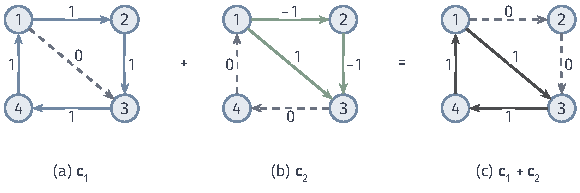
\includegraphics{figures/03-graphs/05-matrices-and-spectra/tikz/incidence-circulation-superposition/figure.pdf}
  \caption{四点五边图上两股环流的叠加$\bm{c}_1+\bm{c}_2$。边旁数字为对应参考方向下的流量分量，虚线表示流量为零。(a) 沿外圈$1\to2\to3\to4\to1$的单位环流$\bm{c}_1$。(b) 沿三角形$1\to3\to2\to1$的单位环流$\bm{c}_2$，其中边$12,23$因逆参考方向而取$-1$。(c) 叠加结果在边$12,23$上正反抵消为零，化为沿三角形$1\to3\to4\to1$的单位环流。}
  \label{fig:incidence-circulation-superposition}
\end{BookInlineFigure}

把“每个顶点处净流出量均为零”这一守恒条件写成一般形式，就得到环流与环空间的严格定义。

\begin{definition}[环流与环空间]
\label{def:graph-cycle-space}
设$\mathcal{G}=(V,E)$为有限图，$\bm{B}\in\mathbb{R}^{n\times m}$为其关联矩阵。若边流量向量$\bm{q}\in\mathbb{R}^E$在每个顶点处的净流出量均为零，即满足
\[
(\bm{B}\bm{q})_v=0\quad(\forall\,v\in V),
\qquad\text{或等价地}\qquad \bm{B}\bm{q}=\bm{0},
\]
则称$\bm{q}$为图$\mathcal{G}$上的一个\term{环流}（circulation）。全体实数环流构成的边空间线性子空间（即关联矩阵$\bm{B}\colon\mathbb{R}^E\to\mathbb{R}^V$的零空间）称为图$\mathcal{G}$的\term{环空间}（cycle space），记为
\begin{equation}
\mathcal{C}(\mathcal{G})=\{\bm{q}\in\mathbb{R}^E:\bm{B}\bm{q}=\bm{0}\}
=\ker\bm{B}.
\label{eq:incidence-cycle-space}
\end{equation}
\end{definition}

需要注意，本章定义的环空间$\mathcal{C}(\mathcal{G})$是实数域$\mathbb{R}$上的线性子空间：每条边可以承载任意实数大小的流量，负分量表示流向与参考方向相反。这与组合图论中在二元域$\mathbb{F}_2$（模$2$加法）下讨论的边子集对称差不同——在实数环空间中，两股同向的单位环流相加会变成$2$倍流量的环流，只有方向相反、大小相等的两股流量叠加才会抵消为零。

一般而言，环空间$\mathcal{C}(\mathcal{G})$中的元素既可以是沿单个简单环绕行的流量，也可以是由多个不同环路按任意实系数线性叠加而成的复合守恒流。那么，任意一个复杂的环流是否都能由少数几个基本简单环线性表出？第~\ref{sec:incidence-fundamental-bases}小节将利用生成森林给出肯定的回答与具体构造方法。在此之前，我们先考察边空间中由沿边差分生成的另一半子空间。

\subsection{割空间}
\label{sec:incidence-cut-space}

现在从相反的方向在边空间$\mathbb{R}^E$中生成向量：先给定顶点函数$\bm{f}\in\mathbb{R}^V$，再通过沿边差分算子$\bm{B}^\top$计算沿边差分向量$\bm{d}=\bm{B}^\top\bm{f}\in\mathbb{R}^E$。

最简单的一类顶点函数是将顶点集$V$分成两部分、在一侧赋$1$而在另一侧赋$0$的指示函数。任取顶点子集$S\subseteq V$，记其补集为$\bar{S}=V\setminus S$，令指示向量$\bm{1}_S\in\mathbb{R}^V$在$S$内的顶点上取$1$、在$\bar{S}$内的顶点上取$0$。对$\bm{1}_S$作用沿边差分算子，得到边空间中的列向量
\[
\bm{d}_S=\bm{B}^\top\bm{1}_S\in\mathbb{R}^E.
\]
对任意一条参考方向为$e\colon u\to v$的边，其分量$(\bm{d}_S)_e=\bm{1}_S(u)-\bm{1}_S(v)$只有三种可能取值：
\begin{itemize}
\item 若$u\in S$且$v\in\bar{S}$（边沿参考方向从$S$穿出到$\bar{S}$），则$(\bm{d}_S)_e=1-0=+1$；
\item 若$u\in\bar{S}$且$v\in S$（边沿参考方向从$\bar{S}$穿入到$S$），则$(\bm{d}_S)_e=0-1=-1$；
\item 若$u,v$同属于$S$或同属于$\bar{S}$（边不跨越割$(S,\bar{S})$），则$(\bm{d}_S)_e=0$。
\end{itemize}
因此，$\bm{d}_S$只在跨越割$(S,\bar{S})$的边上非零，称为对应于顶点子集$S$的\emph{割向量}（或带符号割指示向量）。

以四点五边图上的子集$S=\{1,2\}$及其补集$\bar{S}=\{3,4\}$为例。此时顶点指示向量为$\bm{1}_S=(1,1,0,0)^\top$。按边序$(12,23,34,41,13)$逐条检查五条边的端点位置：边$12$（$1\to2$）两端都在$S$内，差值为$1-1=0$；边$34$（$3\to4$）两端都在$\bar{S}$内，差值为$0-0=0$；边$23$（$2\to3$）和边$13$（$1\to3$）分别从$S$内的顶点$2,1$指向$\bar{S}$内的顶点$3$，差值均为$1-0=+1$；边$41$（$4\to1$）从$\bar{S}$内的$4$指向$S$内的$1$，差值为$0-1=-1$。汇总起来，子集$S=\{1,2\}$生成的割向量为
\[
\bm{d}_S=\bm{B}^\top\bm{1}_S=(0,1,0,-1,1)^\top\in\mathbb{R}^5.
\]
图~\ref{fig:incidence-cut-vector-example}直观展示了这一过程：左图以虚线将顶点集划分为上侧$S=\{1,2\}$（读数$1$）与下侧$\bar{S}=\{3,4\}$（读数$0$）；右图标出经$\bm{B}^\top$作用后各边上的差分分量，内部边$12,34$分量为$0$，三条跨割边$23,41,13$按穿行方向分别取$+1,-1,+1$。

\begin{BookInlineFigure}
  \centering
  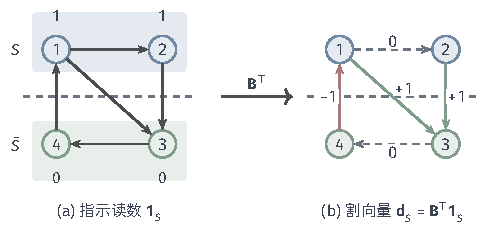
\includegraphics{figures/03-graphs/05-matrices-and-spectra/tikz/incidence-cut-vector-example/figure.pdf}
  \caption{四点五边图上子集$S=\{1,2\}$对应的割向量构造。(a) 将顶点划分为$S=\{1,2\}$（蓝底，赋读数$1$）与$\bar{S}=\{3,4\}$（绿底，赋读数$0$），构成顶点指示向量$\bm{1}_S=(1,1,0,0)^\top$。(b) 经沿边差分算子$\bm{B}^\top$作用后得到的割向量$\bm{d}_S=(0,1,0,-1,1)^\top$：同侧边$12,34$（虚线）差值为$0$，从$S$指向$\bar{S}$的跨割边$23,13$（绿线）取$+1$，从$\bar{S}$指向$S$的跨割边$41$（红线）取$-1$。}
  \label{fig:incidence-cut-vector-example}
\end{BookInlineFigure}

不仅$0$--$1$指示函数如此，任意一个实值顶点函数$\bm{f}\in\mathbb{R}^V$都可以按单点指示向量（即标准基向量$\bm{1}_{\{v\}}=\bm{e}_v$）展开为$\bm{f}=\sum_{v\in V}f(v)\bm{1}_{\{v\}}$。利用矩阵乘法的线性性，它的沿边差分向量可以写成
\[
\bm{B}^\top\bm{f}
=\sum_{v\in V}f(v)\,\bm{B}^\top\bm{1}_{\{v\}}
=\sum_{v\in V}f(v)\,\bm{d}_{\{v\}}.
\]
上式右端每一项都是单点割向量$\bm{d}_{\{v\}}=\bm{B}^\top\bm{1}_{\{v\}}$的数乘。这说明：任意顶点函数的沿边差分向量都是割向量的线性组合；反过来，任意一组割向量的线性组合$\sum_k\alpha_k\bm{B}^\top\bm{1}_{S_k}=\bm{B}^\top\bigl(\sum_k\alpha_k\bm{1}_{S_k}\bigr)$也必定是某个顶点函数的沿边差分向量。由此我们给出割空间的形式化定义。

\begin{definition}[割空间]
\label{def:graph-cut-space}
设$\mathcal{G}=(V,E)$为有限图，$\bm{B}\in\mathbb{R}^{n\times m}$为其关联矩阵。若边向量$\bm{d}\in\mathbb{R}^E$可以表示为某个顶点函数$\bm{f}\in\mathbb{R}^V$的沿边差分向量，即存在$\bm{f}\in\mathbb{R}^V$使得
\[
\bm{d}=\bm{B}^\top\bm{f}\qquad\bigl(\text{即对每条边 }e\colon u\to v\text{ 有 }d_e=f(u)-f(v)\bigr),
\]
则称$\bm{d}$为图$\mathcal{G}$上的一个沿边差分向量（或割差分向量）。全体顶点函数的沿边差分向量构成的边空间线性子空间（即沿边差分算子$\bm{B}^\top\colon\mathbb{R}^V\to\mathbb{R}^E$的像空间）称为图$\mathcal{G}$的\term{割空间}（cut space），记为
\begin{equation}
\mathcal{D}(\mathcal{G})=\{\bm{B}^\top\bm{f}:\bm{f}\in\mathbb{R}^V\}=\operatorname{im}\bm{B}^\top.
\label{eq:incidence-cut-space}
\end{equation}
\end{definition}

\paragraph{正交直和分解}

把定义~\ref{def:graph-cycle-space}与定义~\ref{def:graph-cut-space}放在一起，一个核心几何事实立刻浮现：环空间$\mathcal{C}(\mathcal{G})=\ker\bm{B}$与割空间$\mathcal{D}(\mathcal{G})=\operatorname{im}\bm{B}^\top$在边空间$\mathbb{R}^E$中正交互补。

先验证正交性。任取一个环流$\bm{c}\in\mathcal{C}(\mathcal{G})=\ker\bm{B}$和一个沿边差分向量$\bm{d}=\bm{B}^\top\bm{f}\in\mathcal{D}(\mathcal{G})$。根据式~\eqref{eq:incidence-adjoint-pairing}的伴随恒等式，二者在边空间中的内积为
\[
\langle\bm{d},\bm{c}\rangle_E
=\langle\bm{B}^\top\bm{f},\bm{c}\rangle_E
=\langle\bm{f},\bm{B}\bm{c}\rangle_V
=\langle\bm{f},\bm{0}\rangle_V=0,
\]
其中倒数第二步直接使用了环流的守恒条件$\bm{B}\bm{c}=\bm{0}$。

用简单环路可以直观看出两个向量内积为何恒为零。比如沿三角形$1\to2\to3\to1$绕行一圈的单位环流，将它与任意顶点函数$\bm{f}$的沿边差分作内积，相当于把沿环三步的端点差逐段相加：
\[
\bigl(f(1)-f(2)\bigr)+\bigl(f(2)-f(3)\bigr)+\bigl(f(3)-f(1)\bigr)=0.
\]
环上的每个顶点读数恰好出现两次——在离开该点的一步中取正号，在进入该点的一步中取负号——绕行闭合回路一圈后必然首尾相消（对应物理学中的基尔霍夫电压定律：保守势场沿任意闭合回路的电势降之和为零）。

不仅如此，割空间$\mathcal{D}(\mathcal{G})$的正交补$\mathcal{D}(\mathcal{G})^\perp$恰好就是整个环空间$\mathcal{C}(\mathcal{G})$。事实上，设边向量$\bm{q}\in\mathbb{R}^E$与割空间中的每一个沿边差分向量都正交，即对任意$\bm{f}\in\mathbb{R}^V$都有
\[
0=\langle\bm{B}^\top\bm{f},\bm{q}\rangle_E=\langle\bm{f},\bm{B}\bm{q}\rangle_V.
\]
由于上式对所有顶点函数$\bm{f}\in\mathbb{R}^V$均成立，特别地取$\bm{f}=\bm{B}\bm{q}\in\mathbb{R}^V$，即得
\[
\lVert\bm{B}\bm{q}\rVert_2^2=\langle\bm{B}\bm{q},\bm{B}\bm{q}\rangle_V=0,
\]
从而$\bm{B}\bm{q}=\bm{0}$，说明$\bm{q}\in\ker\bm{B}=\mathcal{C}(\mathcal{G})$。在有限维欧氏空间中，任意子空间与其正交补构成整个空间的正交直和（可参考\BookChapterRef{chap:inner-product-spaces}{卷二"内积空间"章}），因此边空间$\mathbb{R}^E$具有正交直和分解：
\begin{equation}
\mathbb{R}^E=\mathcal{C}(\mathcal{G})\oplus\mathcal{D}(\mathcal{G})
=\ker\bm{B}\oplus\operatorname{im}\bm{B}^\top.
\label{eq:incidence-edge-space-decomposition}
\end{equation}

式~\eqref{eq:incidence-edge-space-decomposition}表明，图上的任意边向量$\bm{q}\in\mathbb{R}^E$都可以唯一地分解为一个守恒环流$\bm{c}\in\mathcal{C}(\mathcal{G})$与一个沿边差分向量$\bm{d}\in\mathcal{D}(\mathcal{G})$之和：$\bm{q}=\bm{c}+\bm{d}$且$\langle\bm{c},\bm{d}\rangle_E=0$。分解的唯一性由正交性直接保证：若另有$\bm{q}=\bm{c}'+\bm{d}'$，相减得$\bm{c}-\bm{c}'=\bm{d}'-\bm{d}$；该差向量同时属于相互正交的$\mathcal{C}(\mathcal{G})$与$\mathcal{D}(\mathcal{G})$，故与自身的内积为零，只能是零向量。

我们用四点五边图上的边向量$\bm{q}=(1,2,1,0,1)^\top$验证这一正交分解：
\[
\bm{q}=\underbrace{(1,1,1,1,0)^\top}_{\bm{c}_1\in\mathcal{C}(\mathcal{G})}
      +\underbrace{(0,1,0,-1,1)^\top}_{\bm{d}_S\in\mathcal{D}(\mathcal{G})},
\]
其中第一项是外圈单位环流$\bm{c}_1$，第二项是子集$S=\{1,2\}$生成的割向量$\bm{d}_S$。容易核对$\langle\bm{c}_1,\bm{d}_S\rangle_E=0+1+0-1+0=0$。例如在边$41$上，环流分量$+1$与割差分分量$-1$叠加后恰好给出$q_{41}=0$；在边$23$上，两项同为$+1$，叠加给出$q_{23}=2$。图~\ref{fig:incidence-flow-decomposition}在三个并排面板中展示了$\bm{q}$、$\bm{c}_1$与$\bm{d}_S$的逐边分量关系。

\begin{BookInlineFigure}
  \centering
  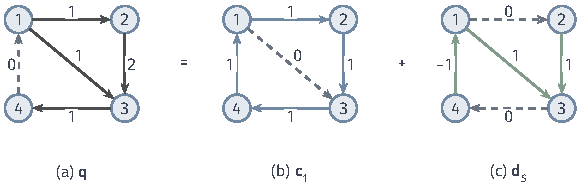
\includegraphics{figures/03-graphs/05-matrices-and-spectra/tikz/incidence-flow-decomposition/figure.pdf}
  \caption{四点五边图上的边向量正交分解$\bm{q}=\bm{c}_1+\bm{d}_S$，其中$S=\{1,2\}$。每条边旁的数值是对应参考方向下的边分量，虚线表示分量为零。}
  \label{fig:incidence-flow-decomposition}
\end{BookInlineFigure}

需要指出的是：虽然边向量$\bm{q}$分解出的沿边差分分量$\bm{d}\in\mathcal{D}(\mathcal{G})$是唯一的，但满足$\bm{B}^\top\bm{f}=\bm{d}$的原像顶点函数$\bm{f}\in\mathbb{R}^V$并不唯一——给$\bm{f}$加上任意属于零空间$\ker\bm{B}^\top$的向量，沿边差分向量$\bm{B}^\top\bm{f}$都保持不变。下一小节通过刻画$\ker\bm{B}^\top$的具体结构，精确算出关联矩阵的秩以及环空间、割空间的维数。

\subsection{子空间维数}
\label{sec:incidence-rank-dimensions}

要计算割空间$\mathcal{D}(\mathcal{G})=\operatorname{im}\bm{B}^\top$与环空间$\mathcal{C}(\mathcal{G})=\ker\bm{B}$各自的维数，关键在于先搞清楚：什么样的顶点函数$\bm{f}\in\mathbb{R}^V$在经过沿边差分算子$\bm{B}^\top$作用后会变成零向量？也就是说，零空间$\ker\bm{B}^\top=\{\bm{f}\in\mathbb{R}^V:\bm{B}^\top\bm{f}=\bm{0}\}$具有什么结构、维数是多少？下面我们分四步把推理过程完整展开。

\paragraph{第一步：同一连通分量内的顶点读数必定相等}

根据沿边差分的定义式~\eqref{eq:incidence-edge-difference}，$\bm{B}^\top\bm{f}=\bm{0}$等价于在每一条边$e\colon u\to v\in E$上都有
\[
f(u)-f(v)=0,\qquad\text{即}\qquad f(u)=f(v).
\]
这表明，只要两个顶点之间有一条边直接相连，它们的读数就必须相等。更进一步，如果两个顶点$i$和$j$属于图的同一个连通分量，那么按连通性的定义，图中存在一条连接$i$与$j$的路径$i=w_0,w_1,\ldots,w_s=j$，其中相邻两步$\{w_{r-1},w_r\}$都是图中的边。沿这条路径逐边应用“相邻端点读数相等”，便得到传递链：
\[
f(i)=f(w_0)=f(w_1)=\cdots=f(w_s)=f(j).
\]
因此，任何满足$\bm{B}^\top\bm{f}=\bm{0}$的顶点函数$\bm{f}$，在图的每一个连通分量内部都必须取同一个常数值。

\paragraph{第二步：不同连通分量之间的常数可以彼此独立选取}

如果整张图$\mathcal{G}$是连通的（只有$1$个连通分量），那么上面第一步已经说明所有$n$个顶点的读数都必须等于同一个常数$\alpha_1$。但如果图$\mathcal{G}$不连通，设它的顶点集$V$划分为$c$个互不相交的连通分量（connected components）：
\[
V=V_1\cup V_2\cup\cdots\cup V_c.
\]
为什么每个连通分量$V_k$可以各自独立地任选一个常数$\alpha_k\in\mathbb{R}$，而不会违反$\bm{B}^\top\bm{f}=\bm{0}$？

原因在于：不同连通分量$V_k$与$V_\ell$（$k\neq\ell$）之间没有任何边相连。换言之，图$\mathcal{G}$中的每一条边$e\colon u\to v\in E$，其两个端点$u$和$v$必定同时落在某一个连通分量$V_k$内部，绝不会出现一端在$V_k$、另一端在$V_\ell$的跨分量边。于是，只要我们在第$1$个连通分量$V_1$的所有顶点上统一赋常数$\alpha_1$，在第$2$个连通分量$V_2$的所有顶点上统一赋常数$\alpha_2$，……，在第$c$个连通分量$V_c$的所有顶点上统一赋常数$\alpha_c$，那么对任意一条边$e\colon u\to v$（不妨设它落在$V_k$内），两端的读数差就恒为
\[
f(u)-f(v)=\alpha_k-\alpha_k=0.
\]
至于其他分量$V_\ell$（$\ell\neq k$）上选了什么常数$\alpha_\ell$，没有边把$\alpha_\ell$和$\alpha_k$连起来作差，因此$\alpha_1,\alpha_2,\ldots,\alpha_c$这$c$个实数彼此之间没有任何耦合约束，可以完全独立地任意取值。特别地，若图中某个顶点$v$是不连任何边的孤立顶点（isolated vertex），它自己单独构成一个连通分量$V_k=\{v\}$；由于没有任何边以$v$为端点，$f(v)=\alpha_k$不出现在$\bm{B}^\top\bm{f}$的任何分量中，也可以独立任取一个实数。

\paragraph{第三步：用分量指示向量表示零空间$\ker\bm{B}^\top$}

为了把“在每个连通分量$V_k$上各自独立取常数$\alpha_k$”写成标准的线性代数语言，我们对第$k$个连通分量$V_k$（$k=1,\ldots,c$）定义其\emph{分量指示向量}$\bm{1}_{V_k}\in\mathbb{R}^V$：
\[
(\bm{1}_{V_k})_v=
\begin{cases}
1,& v\in V_k,\\
0,& v\notin V_k.
\end{cases}
\]
这样，给第$k$个分量的所有顶点赋常数$\alpha_k$，合在一起写成列向量就是线性组合
\begin{equation}
\bm{f}=\alpha_1\bm{1}_{V_1}+\alpha_2\bm{1}_{V_2}+\cdots+\alpha_c\bm{1}_{V_c}.
\label{eq:incidence-ker-bt-expansion}
\end{equation}
我们来逐坐标核对式~\eqref{eq:incidence-ker-bt-expansion}：任取图中的一个顶点$v\in V$，因为$V=V_1\cup\cdots\cup V_c$是互不相交的划分，$v$恰好属于唯一的一个连通分量$V_k$。在顶点$v$所在的坐标位置上，只有$\bm{1}_{V_k}$取$1$，其余$c-1$个指示向量$\bm{1}_{V_\ell}$（$\ell\neq k$）全部取$0$，因此式~\eqref{eq:incidence-ker-bt-expansion}右端在顶点$v$处的值恰好是
\[
\alpha_1\cdot 0+\cdots+\alpha_k\cdot 1+\cdots+\alpha_c\cdot 0=\alpha_k=f(v).
\]
这证明了：$\bm{f}\in\ker\bm{B}^\top$当且仅当$\bm{f}$可以写成式~\eqref{eq:incidence-ker-bt-expansion}的形式。也就是说，这$c$个分量指示向量$\{\bm{1}_{V_1},\ldots,\bm{1}_{V_c}\}$张成了整个零空间$\ker\bm{B}^\top$。

\paragraph{第四步：证明$c$个分量指示向量线性无关}

要确认$\{\bm{1}_{V_1},\ldots,\bm{1}_{V_c}\}$构成$\ker\bm{B}^\top$的一组基，还需证明它们线性无关。设有一组实系数$\alpha_1,\ldots,\alpha_c\in\mathbb{R}$使线性组合等于零向量：
\[
\alpha_1\bm{1}_{V_1}+\alpha_2\bm{1}_{V_2}+\cdots+\alpha_c\bm{1}_{V_c}=\bm{0}.
\]
对任意下标$k\in\{1,\ldots,c\}$，连通分量$V_k$都是非空顶点子集，我们在$V_k$中任取一个代表顶点$v\in V_k$，读取上式左右两端在第$v$个坐标处的分量：左端等于$\alpha_k$，右端等于零向量的分量$0$，故必有$\alpha_k=0$。由于$k$是任意的，全部系数$\alpha_1=\alpha_2=\cdots=\alpha_c=0$。这证明了$\{\bm{1}_{V_1},\ldots,\bm{1}_{V_c}\}$线性无关，从而构成$\ker\bm{B}^\top$的一组基，零空间的维数恰等于连通分量个数$c$：
\[
\dim\ker\bm{B}^\top=c.
\]

我们用一个具体例子配合图~\ref{fig:incidence-component-constants}来直观核对上述推理。考虑由$n=5$个顶点、$c=2$个连通分量组成的图：第一个分量$V_1=\{1,2,3\}$是一个三角形，第二个分量$V_2=\{4,5\}$是一条独立边。两个分量的指示向量分别为
\[
\bm{1}_{V_1}=(1,1,1,0,0)^\top,\qquad
\bm{1}_{V_2}=(0,0,0,1,1)^\top.
\]
它们的任意线性组合为
\[
\bm{f}=\alpha_1\bm{1}_{V_1}+\alpha_2\bm{1}_{V_2}
=(\alpha_1,\alpha_1,\alpha_1,\alpha_2,\alpha_2)^\top.
\]
如图~\ref{fig:incidence-component-constants}(c)所示，三角形内部三条边的两端读数均为$\alpha_1$，差值为$\alpha_1-\alpha_1=0$；底边$\{4,5\}$的两端读数均为$\alpha_2$，差值为$\alpha_2-\alpha_2=0$；而$V_1$与$V_2$之间没有边相连，$\alpha_1$与$\alpha_2$永远不会被放在同一条边上相减。若令$\bm{f}=(0,0,0,0,0)^\top$，从顶点$1$读出$\alpha_1=0$，从顶点$4$读出$\alpha_2=0$，两个指示向量显然线性无关，张成二维零空间$\ker\bm{B}^\top$。

\begin{BookInlineFigure}
  \centering
  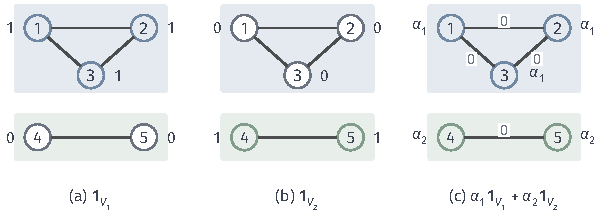
\includegraphics{figures/03-graphs/05-matrices-and-spectra/tikz/incidence-component-constants/figure.pdf}
  \caption{含$c=2$个连通分量$V_1=\{1,2,3\}$（蓝底）与$V_2=\{4,5\}$（绿底）的五点图上$\ker\bm{B}^\top$的基与通解。(a) 第一分量指示向量$\bm{1}_{V_1}=(1,1,1,0,0)^\top$。(b) 第二分量指示向量$\bm{1}_{V_2}=(0,0,0,1,1)^\top$。(c) 一般零空间向量$\bm{f}=\alpha_1\bm{1}_{V_1}+\alpha_2\bm{1}_{V_2}$在两个分量上分别取独立常数$\alpha_1,\alpha_2$，每条边的两端同属一个分量，沿边差分全为$0$。}
  \label{fig:incidence-component-constants}
\end{BookInlineFigure}

有了$\dim\ker\bm{B}^\top=c$，连续使用两次线性代数的秩零度定理（rank-nullity theorem），即可直接导出关联矩阵的秩以及割空间、环空间的维数公式。

\begin{theorem}[环空间与割空间的维数]
\label{thm:incidence-cycle-cut-dimensions}
设有限图$\mathcal{G}=(V,E)$有$n$个顶点、$m$条边和$c$个连通分量，关联矩阵为$\bm{B}\in\mathbb{R}^{n\times m}$。则关联矩阵的秩为
\begin{equation}
\operatorname{rank}\bm{B}=\operatorname{rank}\bm{B}^\top=n-c,
\label{eq:incidence-rank-components}
\end{equation}
且割空间$\mathcal{D}(\mathcal{G})=\operatorname{im}\bm{B}^\top$与环空间$\mathcal{C}(\mathcal{G})=\ker\bm{B}$的维数分别为
\begin{equation}
\dim\mathcal{D}(\mathcal{G})=n-c,\qquad
\dim\mathcal{C}(\mathcal{G})=m-n+c.
\label{eq:incidence-cycle-cut-dimensions}
\end{equation}
\end{theorem}

\begin{proof}
首先考察沿边差分算子$\bm{B}^\top\colon\mathbb{R}^V\to\mathbb{R}^E$。它的定义域是$n$维顶点空间$\mathbb{R}^V$，零空间$\ker\bm{B}^\top$由$c$个连通分量的指示向量$\{\bm{1}_{V_1},\ldots,\bm{1}_{V_c}\}$张成且线性无关，故$\dim\ker\bm{B}^\top=c$。对线性映射$\bm{B}^\top$应用秩零度定理，其像空间$\mathcal{D}(\mathcal{G})=\operatorname{im}\bm{B}^\top$的维数为
\[
\dim\mathcal{D}(\mathcal{G})=\operatorname{rank}\bm{B}^\top=\dim\mathbb{R}^V-\dim\ker\bm{B}^\top=n-c.
\]
由于矩阵与其转置的秩相等，有$\operatorname{rank}\bm{B}=\operatorname{rank}\bm{B}^\top=n-c$，式~\eqref{eq:incidence-rank-components}得证。

再考察净流出汇总算子$\bm{B}\colon\mathbb{R}^E\to\mathbb{R}^V$。它的定义域是$m$维边空间$\mathbb{R}^E$，秩为$\operatorname{rank}\bm{B}=n-c$。对$\bm{B}$应用秩零度定理，其零空间$\mathcal{C}(\mathcal{G})=\ker\bm{B}$的维数为
\[
\dim\mathcal{C}(\mathcal{G})=\dim\ker\bm{B}=\dim\mathbb{R}^E-\operatorname{rank}\bm{B}=m-(n-c)=m-n+c.
\]
式~\eqref{eq:incidence-cycle-cut-dimensions}得证。
\end{proof}

验证两个具体情形：在图~\ref{fig:incidence-running-example}的四点五边图上，$n=4,m=5,c=1$，由定理~\ref{thm:incidence-cycle-cut-dimensions}立得割空间维数为$4-1=3$，环空间维数为$5-4+1=2$，两者之和$3+2=5=m$，与正交直和分解式~\eqref{eq:incidence-edge-space-decomposition}完全吻合。

又若图$\mathcal{G}$是一片不含任何环的森林（forest），则边数恰为$m=n-c$，此时环空间维数$\dim\mathcal{C}(\mathcal{G})=(n-c)-n+c=0$，即森林上不存在任何非零环流。直观上，无环图中任何非零流量一旦沿某条边流出，最终必然到达度为$1$的叶子顶点而无法绕回，从而在叶子处破坏流量守恒。下一小节将利用生成森林把这一观察转化为显式基的构造与证明。

\subsection{基本环基}
\label{sec:incidence-fundamental-bases}

定理~\ref{thm:incidence-cycle-cut-dimensions}给出了环空间维数$m-n+c$和割空间维数$n-c$，但还没有具体指明怎样找出一组基向量。注意到在一张有$n$个顶点、$c$个连通分量的图$\mathcal{G}=(V,E)$中，任取一棵生成森林$F\subseteq E$（当图连通、$c=1$时就是一棵生成树$T$），森林$F$中包含的\emph{树边}（tree edges）条数恰好是$n-c$，等于割空间的维数；而留在森林之外的\emph{非树边}（non-tree edges，也称弦，$E\setminus F$）条数恰好是$m-(n-c)=m-n+c$，等于环空间的维数。

这并非巧合：用每条非树边与树路径闭合，可以逐一构造出$m-n+c$个线性无关的基本环向量；下一小节再逐一删去每条树边将生成树切成两半，构造出$n-c$个线性无关的基本割向量。

下面说明如何由生成森林$F$和每一条非树边$e\in E\setminus F$构造基本环向量。取定一条非树边$e\colon u\to v\in E\setminus F$，由于$e$的两个端点$u$和$v$属于同一个连通分量，在生成森林$F$内部已经存在唯一一条连接$v$到$u$的树路径$P_e\subseteq F$；将非树边$e$添入$F$中，边集$P_e\cup\{e\}$就构成唯一一个简单环，记为$C_e$。规定沿环$C_e$的绕行方向与非树边$e$本身的参考方向$u\to v$一致（即先沿$e$从$u$走到$v$，再沿树路径$P_e$从$v$走回$u$），据此定义一个边流量向量$\bm{c}^{(e)}\in\mathbb{R}^E$：
\[
\bigl(\bm{c}^{(e)}\bigr)_{e'}=
\begin{cases}
+1,& e'=e\text{（即该非树边本身）},\\[2pt]
+1,& e'\in P_e\text{ 且 }e'\text{ 的参考方向与 }C_e\text{ 的绕行方向一致},\\[2pt]
-1,& e'\in P_e\text{ 且 }e'\text{ 的参考方向与 }C_e\text{ 的绕行方向相反},\\[2pt]
0,& e'\notin C_e\text{（包括其余所有非树边及不在 }P_e\text{ 上的树边）}.
\end{cases}
\]
向量$\bm{c}^{(e)}$称为对应于非树边$e$的\term{基本环}向量（fundamental cycle vector）。

我们在图~\ref{fig:incidence-running-example}的四点五边图上演示这一构造过程。如图~\ref{fig:incidence-fundamental-cycles}(a)所示，选取路径生成树$T=\{12,23,34\}$（共$n-1=3$条树边），留下的两条非树边为$E\setminus T=\{41,13\}$（共$m-n+1=2$条非树边）。

先添入非树边$41$（参考方向$4\to1$）：如图~\ref{fig:incidence-fundamental-cycles}(b)所示，沿非树边$41$从$4$走到$1$，再沿树路径$1\to2\to3\to4$返回$4$。沿途经过的三条树边$12,23,34$均与各自的参考方向同向（各取$+1$），另一条非树边$13$不在环上（取$0$），按边序$(12,23,34,41,13)$得到第一个基本环向量
\[
\bm{c}_1=\bm{c}^{(41)}=(1,1,1,\;1,0)^\top.
\]
再添入非树边$13$（参考方向$1\to3$）：如图~\ref{fig:incidence-fundamental-cycles}(c)所示，沿非树边$13$从$1$走到$3$，再沿树路径$3\to2\to1$返回$1$。返回途中经过的树边$23$和$12$均与各自的参考方向（$2\to3$和$1\to2$）相反，分量均取$-1$；树边$34$和另一条非树边$41$不在环上，均取$0$，得到第二个基本环向量
\[
\bm{c}_2=\bm{c}^{(13)}=(-1,-1,0,\;0,1)^\top.
\]

\begin{BookInlineFigure}
  \centering
  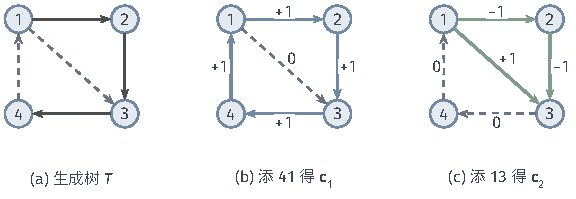
\includegraphics{figures/03-graphs/05-matrices-and-spectra/tikz/incidence-fundamental-cycles/figure.pdf}
  \caption{在四点五边图上由路径生成树$T=\{12,23,34\}$构造基本环基。(a) 实线为三条树边$12,23,34$，虚线为两条非树边$41,13$。(b) 添入非树边$41$并沿树路径$1\to2\to3\to4$闭合，得到基本环向量$\bm{c}_1=(1,1,1,1,0)^\top$。(c) 添入非树边$13$并沿树路径$3\to2\to1$闭合（逆参考方向经过$23$与$12$），得到基本环向量$\bm{c}_2=(-1,-1,0,0,1)^\top$。}
  \label{fig:incidence-fundamental-cycles}
\end{BookInlineFigure}

观察$\bm{c}_1$和$\bm{c}_2$在最后两个坐标——即两条非树边$(41,13)$——上的取值：$\bm{c}_1$在$(41,13)$处为$(1,0)^\top$，$\bm{c}_2$在$(41,13)$处为$(0,1)^\top$，拼在一起恰好是$2\times 2$单位矩阵$\bigl(\begin{smallmatrix}1&0\\0&1\end{smallmatrix}\bigr)$。每条非树边只出现在它自己生成的那个基本环中，而在其他所有基本环中坐标全为$0$。正是这一“非树边坐标呈单位阵”的结构，使基本环向量的线性无关性与坐标展开变得可以直接验证。

\begin{theorem}[基本环基]
\label{thm:incidence-fundamental-cycle-basis}
设有限图$\mathcal{G}=(V,E)$有$n$个顶点、$m$条边和$c$个连通分量，$F\subseteq E$为其一棵生成森林。则由$m-n+c$条非树边$e\in E\setminus F$构造的基本环向量集合
\[
\bigl\{\bm{c}^{(e)}:e\in E\setminus F\bigr\}
\]
构成环空间$\mathcal{C}(\mathcal{G})=\ker\bm{B}$的一组基。特别地，任意环流$\bm{q}\in\mathcal{C}(\mathcal{G})$均可按其在非树边上的分量唯一展开为
\begin{equation}
\bm{q}=\sum_{e\in E\setminus F}q_e\,\bm{c}^{(e)}.
\label{eq:incidence-fundamental-cycle-expansion}
\end{equation}
\end{theorem}

\begin{proof}
我们分三步证明：（1）每个$\bm{c}^{(e)}$属于$\mathcal{C}(\mathcal{G})$；（2）这$m-n+c$个向量线性无关；（3）任意环流$\bm{q}\in\mathcal{C}(\mathcal{G})$均满足展开式~\eqref{eq:incidence-fundamental-cycle-expansion}。

\textbf{第一步（属于环空间）}：对每条非树边$e\in E\setminus F$，$C_e$是一个简单闭合回路。不在$C_e$上的顶点关联的边流量全为$0$，净流出量为$0$；在$C_e$上的每个顶点恰好作为$C_e$中一条边的流入端和另一条边的流出端，按绕行方向一进一出各$1$个单位，根据关联矩阵作用公式~\eqref{eq:incidence-net-outflow}，其净流出量也为$1-1=0$。因此$\bm{B}\bm{c}^{(e)}=\bm{0}$，即$\bm{c}^{(e)}\in\mathcal{C}(\mathcal{G})$。

\textbf{第二步（线性无关）}：设有一组实系数$\{\alpha_e:e\in E\setminus F\}$使得
\[
\sum_{e'\in E\setminus F}\alpha_{e'}\,\bm{c}^{(e')}=\bm{0}.
\]
任取一条非树边$e\in E\setminus F$，读取上式两端在第$e$条边上的坐标分量。由基本环向量的构造规则，$\bm{c}^{(e)}$在边$e$上的分量为$1$，而其余所有基本环向量$\bm{c}^{(e')}$（$e'\neq e$）在非树边$e$上的分量全为$0$。因此上式左端在第$e$条边上的分量就是$\alpha_e\cdot 1+0=\alpha_e$，右端为$0$，故$\alpha_e=0$。对每条非树边$e\in E\setminus F$均如此，说明$\{\bm{c}^{(e)}:e\in E\setminus F\}$线性无关。

\textbf{第三步（张成性与唯一展开式）}：由定理~\ref{thm:incidence-cycle-cut-dimensions}，环空间的维数为$\dim\mathcal{C}(\mathcal{G})=m-n+c$，因此$\mathcal{C}(\mathcal{G})$中$m-n+c$个线性无关的向量已经构成一组基。为了直接导出展开式~\eqref{eq:incidence-fundamental-cycle-expansion}，任取环流$\bm{q}\in\ker\bm{B}$，直接用$\bm{q}$在各条非树边上的分量$q_e$作系数，构造余量向量
\[
\bm{r}=\bm{q}-\sum_{e\in E\setminus F}q_e\,\bm{c}^{(e)}.
\]
一方面，$\bm{r}$是环流的线性组合，故仍满足守恒条件$\bm{B}\bm{r}=\bm{0}$；另一方面，在每一条非树边$e\in E\setminus F$上，$r_e=q_e-q_e\cdot 1=0$。这意味着守恒流$\bm{r}$在所有非树边上全为零，只可能在生成森林$F$的树边上非零。

若$\bm{r}\neq\bm{0}$，设$F'\subseteq F$为$r_{e'}\neq 0$的树边子集。因为$F'$是森林的非空子图（无环），$F'$中必然存在一个只与$F'$中唯一一条边$e_1\in F'$相连的叶子顶点$v$。但在顶点$v$处，$\bm{r}$在关联于$v$的其余所有边上分量皆为$0$，故净流出量为$(\bm{B}\bm{r})_v=\pm r_{e_1}$；由守恒条件$(\bm{B}\bm{r})_v=0$立得$r_{e_1}=0$，与$e_1\in F'$矛盾。（等价地，从生成森林$F$的叶子顶点开始逐次剥去叶子与所连树边，每一步叶子处的守恒方程都迫使该树边流量为零，直至整片森林清空。）因此必有$\bm{r}=\bm{0}$，式~\eqref{eq:incidence-fundamental-cycle-expansion}得证。
\end{proof}

\subsection{基本割基}
\label{sec:incidence-fundamental-cut-bases}

与非树边生成基本环对偶，生成森林$F$中的每一条树边$e\in F$都可以用来构造一个基本割向量。取定一条树边$e\colon u\to v\in F$，设它属于连通分量$V_k$的生成树$T_k$。因为树是连通无环图，从$T_k$中删去树边$e$后，$T_k$恰好分裂成两棵互不连通的子树；取包含边$e$尾端$u$的那棵子树的顶点集为$S_e$（头端$v$落在另一侧$V\setminus S_e$中），以子集$S_e$的指示向量$\bm{1}_{S_e}\in\mathbb{R}^V$作用沿边差分算子$\bm{B}^\top$，定义
\[
\bm{d}^{(e)}=\bm{B}^\top\bm{1}_{S_e}\in\mathbb{R}^E.
\]
考察$\bm{d}^{(e)}$在各条边上的分量：在被删的树边$e\colon u\to v$本身上，尾端$u\in S_e$（读数$1$）、头端$v\notin S_e$（读数$0$），故$\bigl(\bm{d}^{(e)}\bigr)_e=1-0=+1$；在生成森林的其余所有树边$e'\in F\setminus\{e\}$上，删去$e$并没有切断$e'$，因此$e'$的两个端点必定同在$S_e$内或同在$S_e$外，两端读数相等，故$\bigl(\bm{d}^{(e)}\bigr)_{e'}=0$；在原图的非树边$e''\in E\setminus F$上，若$e''$跨越$S_e$与$V\setminus S_e$，则按参考方向从$S_e$穿出取$+1$、穿入取$-1$，不跨割则取$0$。向量$\bm{d}^{(e)}$称为对应于树边$e\in F$的\term{基本割}向量（fundamental cut vector）。

仍在四点五边图的路径生成树$T=\{12,23,34\}$上逐一构造全部$n-1=3$个基本割向量（边序仍为$12,23,34,41,13$），如图~\ref{fig:incidence-tree-cycle-cut}所示。

删去树边$12$（$1\to2$）时（图~\ref{fig:incidence-tree-cycle-cut}(a)），树$T$分裂为尾端侧$S_1=\{1\}$与头端侧$\bar{S}_1=\{2,3,4\}$，树边$12$从$S_1$指向$\bar{S}_1$（取$+1$），其余两条树边$23,34$两端都在$\bar{S}_1$内（取$0$），非树边$41$从$4$指向$1$（取$-1$），非树边$13$从$1$指向$3$（取$+1$），得到第一个基本割向量$\bm{d}_1=\bm{d}^{(12)}$。

删去树边$23$（$2\to3$）时（图~\ref{fig:incidence-tree-cycle-cut}(b)），树$T$分裂为$S_2=\{1,2\}$与$\bar{S}_2=\{3,4\}$，树边$23$取$+1$、树边$12,34$取$0$，非树边$41$取$-1$、$13$取$+1$，得到第二个基本割向量$\bm{d}_2=\bm{d}^{(23)}$。

删去树边$34$（$3\to4$）时（图~\ref{fig:incidence-tree-cycle-cut}(c)），树$T$分裂为$S_3=\{1,2,3\}$与$\bar{S}_3=\{4\}$，树边$34$取$+1$、树边$12,23$取$0$，非树边$41$从$4$进入$1$（取$-1$），非树边$13$两端都在$S_3$内（取$0$），得到第三个基本割向量$\bm{d}_3=\bm{d}^{(34)}$。三个基本割向量依次为
\[
\bm{d}_1=(1,0,0,\;-1,1)^\top,\quad
\bm{d}_2=(0,1,0,\;-1,1)^\top,\quad
\bm{d}_3=(0,0,1,\;-1,0)^\top.
\]

\begin{BookInlineFigure}
  \centering
  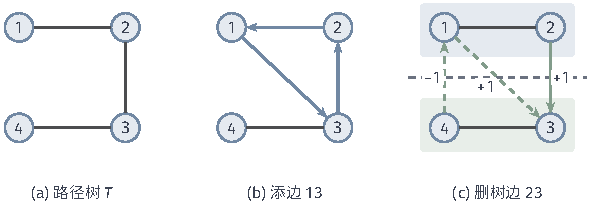
\includegraphics{figures/03-graphs/05-matrices-and-spectra/tikz/incidence-tree-cycle-cut/figure.pdf}
  \caption{在四点五边图上由路径生成树$T=\{12,23,34\}$构造三个基本割基向量。每个面板删去一条树边，蓝底标出含该树边尾端的子树顶点集$S_k$，绿底标出另一侧$\bar{S}_k$；绿实线（$+1$）和红实线（$-1$）为跨割边，灰虚线（$0$）为同侧边。(a) 删树边$12$，$S_1=\{1\}$，得$\bm{d}_1=(1,0,0,-1,1)^\top$。(b) 删树边$23$，$S_2=\{1,2\}$，得$\bm{d}_2=(0,1,0,-1,1)^\top$。(c) 删树边$34$，$S_3=\{1,2,3\}$，得$\bm{d}_3=(0,0,1,-1,0)^\top$。}
  \label{fig:incidence-tree-cycle-cut}
\end{BookInlineFigure}

观察$\bm{d}_1,\bm{d}_2,\bm{d}_3$在前三个坐标——即三条树边$(12,23,34)$——上的取值：它们依次为$(1,0,0)^\top,(0,1,0)^\top,(0,0,1)^\top$，拼在一起恰好是$3\times 3$单位矩阵。每条树边只出现在删去它自己时生成的那个基本割中，而在其余基本割中分量全为$0$。据此可立即证明基本割基定理。

\begin{theorem}[基本割基]
\label{thm:incidence-fundamental-cut-basis}
设有限图$\mathcal{G}=(V,E)$有$n$个顶点、$m$条边和$c$个连通分量，$F\subseteq E$为其一棵生成森林。则由$n-c$条树边$e\in F$构造的基本割向量集合
\[
\bigl\{\bm{d}^{(e)}:e\in F\bigr\}
\]
构成割空间$\mathcal{D}(\mathcal{G})=\operatorname{im}\bm{B}^\top$的一组基。特别地，任意割差分向量$\bm{d}\in\mathcal{D}(\mathcal{G})$均可按其在树边上的分量唯一展开为
\begin{equation}
\bm{d}=\sum_{e\in F}d_e\,\bm{d}^{(e)}.
\label{eq:incidence-fundamental-cut-expansion}
\end{equation}
\end{theorem}

\begin{proof}
首先，每个$\bm{d}^{(e)}=\bm{B}^\top\bm{1}_{S_e}$由顶点函数$\bm{1}_{S_e}$经$\bm{B}^\top$作用生成，故属于$\mathcal{D}(\mathcal{G})=\operatorname{im}\bm{B}^\top$。

其次证明线性无关。设有一组实系数$\{\beta_e:e\in F\}$使得
\[
\sum_{e'\in F}\beta_{e'}\,\bm{d}^{(e')}=\bm{0}.
\]
任取一条树边$e\in F$，读取上式两端在第$e$条边上的坐标分量。由基本割向量的构造规则，$\bm{d}^{(e)}$在树边$e$上的分量为$1$，而其余所有基本割向量$\bm{d}^{(e')}$（$e'\in F\setminus\{e\}$）在树边$e$上的分量全为$0$。因此左端在树边$e$处的分量就是$\beta_e\cdot 1+0=\beta_e$，右端为$0$，故$\beta_e=0$。这证明了$n-c$个基本割向量线性无关。

最后，由定理~\ref{thm:incidence-cycle-cut-dimensions}知割空间的维数为$\dim\mathcal{D}(\mathcal{G})=n-c$。在$n-c$维空间中，$n-c$个线性无关的向量$\{\bm{d}^{(e)}:e\in F\}$必然构成一组基。因此，任意$\bm{d}\in\mathcal{D}(\mathcal{G})$都可唯一展开为$\bm{d}=\sum_{e'\in F}\beta_{e'}\bm{d}^{(e')}$；读取两端在每条树边$e\in F$上的坐标分量，立得$d_e=\beta_e$，即展开式~\eqref{eq:incidence-fundamental-cut-expansion}成立。
\end{proof}

\paragraph{正交性的验证}

我们可以用四点五边图上求出的基本环基$\{\bm{c}_1,\bm{c}_2\}$与基本割基$\{\bm{d}_1,\bm{d}_2,\bm{d}_3\}$直接核对环空间与割空间的正交性。例如，取基本割向量$\bm{d}_2=(0,1,0,-1,1)^\top$，将其分别与$\bm{c}_1$和$\bm{c}_2$作内积：
\[
\begin{aligned}
\bm{c}_1^\top\bm{d}_2&=1\cdot0+1\cdot1+1\cdot0+1\cdot(-1)+0\cdot1=1-1=0,\\
\bm{c}_2^\top\bm{d}_2&=(-1)\cdot0+(-1)\cdot1+0\cdot0+0\cdot(-1)+1\cdot1=-1+1=0.
\end{aligned}
\]
从图上看，任何一个基本环一旦跨过基本割从$S_e$进入$\bar{S}_e$（贡献一次树边或非树边同向乘积），为了回到起点就必须再次跨过该割从$\bar{S}_e$返回$S_e$（贡献一次反向乘积），两次跨割的乘积符号相反、恰好成对抵消。

最后指出，换选另一棵生成树（或生成森林）会得到另一套基本环基和基本割基，基向量的具体坐标随之改变；但它们所张成的环空间$\mathcal{C}(\mathcal{G})=\ker\bm{B}$和割空间$\mathcal{D}(\mathcal{G})=\operatorname{im}\bm{B}^\top$本身只由原图的关联矩阵$\bm{B}$唯一确定，不随生成树的选择而改变。

\section{全幺模性}
\label{sec:graph-incidence-total-unimodularity}
\label{sec:incidence-tu-definition}

前面两节建立了顶点函数和边函数的空间，并给出了正交分解和维数。现在转向另一个问题：如果把图上的流量或选边写成线性规划，什么时候即使放开整数约束，最优解仍然是整数？答案取决于系数矩阵的方子式——这就是全幺模性。

举一个小例子。矩阵
\[
\bm{M}=\begin{pmatrix}1&1\\1&-1\end{pmatrix}
\]
的每个条目都是$\pm1$，但$\det\bm{M}=1\cdot(-1)-1\cdot1=-2$。以$(1,0)^\top$为右端解方程$\bm{M}\bm{x}=(1,0)^\top$，克莱姆法则给出
\[
x_1=\frac{\det\begin{pmatrix}1&1\\0&-1\end{pmatrix}}{\det\bm{M}}=\frac{-1}{-2}=\frac{1}{2},\qquad
x_2=\frac{\det\begin{pmatrix}1&1\\1&0\end{pmatrix}}{\det\bm{M}}=\frac{-1}{-2}=\frac{1}{2}.
\]
分母$-2$正是行列式的值。只要行列式不是$\pm1$，这种除法就可能产生分数。

全幺模性从根本上排除这个问题：它要求从矩阵中取出任意方形子矩阵时，所得行列式都属于$\{0,1,-1\}$。

\begin{definition}[全幺模矩阵]
\label{def:graph-total-unimodularity}
若矩阵的每个方形子矩阵的行列式都属于$\{0,1,-1\}$，就称它为\term{全幺模矩阵}（totally unimodular matrix，简称TUM）。
\end{definition}

取一阶方子式就是单个条目，因此全幺模矩阵的每个元素只能是$0$、$1$或$-1$。但上面的$\bm{M}$说明，仅检查条目远远不够——还必须检查所有更高阶的方子式。

\subsection{带符号关联矩阵的全幺模性}
\label{sec:incidence-signed-tu}

前一节定义的关联矩阵$\bm{B}$，每一列在尾端取$+1$、头端取$-1$，其余为零。这种矩阵称为\term{带符号关联矩阵}（signed incidence matrix）。无向图只需为每条边选一个记录方向；反转一条边只让相应列变号，而列变号不改变任何方子式的绝对值，所以全幺模性与方向选择无关。

\begin{theorem}[带符号关联矩阵]
\label{thm:graph-signed-incidence-tu}
有限无自环图的带符号关联矩阵是全幺模矩阵。
\end{theorem}

\begin{proof}
对方子式的阶数$k$做归纳。

$k=1$时，条目本身属于$\{0,1,-1\}$，满足条件。

设所有低于$k$阶的方子式已满足结论，考察$\bm{B}$中任意$k$行$k$列组成的方阵。按这个方阵中各列的结构，分三种情形讨论。

情形一：有一列在方阵中没有保留任何端点行。这一列全为零，含有零列的方阵行列式为零。

情形二：有一列只保留了一个端点行。这一列中唯一的非零元为$+1$或$-1$。沿这一列展开行列式，得到这个$\pm1$乘以一个$(k-1)$阶的余子式。由归纳假设，余子式属于$\{0,1,-1\}$，两者相乘仍属于$\{0,1,-1\}$。

情形三：每一列的两个端点行都保留了下来。此时每列恰有一个$+1$和一个$-1$，列和为零。把方阵的所有行相加，得到零行向量。行向量线性相关意味着行列式为零。

三种情形涵盖了所有可能的列结构，归纳完毕。
\end{proof}

用一个具体的例子来看证明是怎样起作用的。以无向三角形为例，按$1\to2$、$2\to3$、$3\to1$记录方向，关联矩阵为
\[
\bm{B}_\triangle=
\begin{pmatrix}
1&0&-1\\
-1&1&0\\
0&-1&1
\end{pmatrix}.
\]
三行之和为零向量，因此整体行列式为零——这正是情形三。再看左上角的$2\times2$子矩阵$\bigl(\begin{smallmatrix}1&0\\-1&1\end{smallmatrix}\bigr)$：其中第一列只保留了一个端点行（情形二），沿该列展开得到行列式$1$。

注意三角形含有奇数长的环，但这并不影响带符号关联矩阵的全幺模性。证明中用到的只是"每列有一个$+1$和一个$-1$"这个结构性质，与环的奇偶无关。

从$\bm{B}$中删掉若干行后，剩余矩阵的每个方子式仍然是原矩阵的某个方子式。因此约化后的矩阵也全幺模——后面讨论线性规划时删去冗余守恒式会用到这一点。

\subsection{无符号关联矩阵的全幺模性}
\label{sec:incidence-unsigned-tu}

如果只想记录一条边接在哪两个顶点，不需要区分出入方向，就在两个端点对应的行各填一个$1$，其余行填零。按这个规则得到的矩阵$\bm{N}$称为\term{无符号关联矩阵}（unsigned incidence matrix）。

仍用三角形，边序不变。无符号关联矩阵为
\[
\bm{N}_\triangle=
\begin{pmatrix}
1&0&1\\
1&1&0\\
0&1&1
\end{pmatrix}.
\]
与带符号版本的唯一区别是第三列第一行从$-1$变成了$+1$。计算行列式：沿第一行展开，
\[
\det\bm{N}_\triangle=1\cdot(1\cdot1-0\cdot1)-0+1\cdot(1\cdot1-1\cdot0)=1+1=2.
\]
同一张图在两种端点符号约定下产生了不同的行列式值。

\begin{theorem}[无符号关联矩阵]
\label{thm:graph-unsigned-incidence-tu}
有限简单无向图的无符号关联矩阵全幺模，当且仅当该图是二部图。
\end{theorem}

\begin{proof}
先证充分性。若图是二部图，顶点分为两侧$U$和$W$，每条边都连接两侧。把$W$侧对应的所有行乘以$-1$。每一列原先在两个端点都是$+1$，变号后$U$侧的端点留下$+1$，$W$侧的端点变成$-1$。这恰好是把所有边统一从$U$指向$W$得到的带符号关联矩阵。行变号不改变方子式的绝对值（每变号一行使行列式乘$-1$，多行变号的效果相乘）。因此由定理~\ref{thm:graph-signed-incidence-tu}可知原矩阵也全幺模。

再证必要性。若图不是二部图，则存在奇数长度的环。设这个环按顶点$1,2,\ldots,\ell$的次序闭合，$\ell$为奇数。只选这$\ell$个顶点的行和环上$\ell$条边的列（即边$\{1,2\},\{2,3\},\ldots,\{\ell,1\}$），得到一个$\ell\times\ell$方阵。

对这个方阵的行列式作排列展开。每列对应环上的一条边，恰好在两行上有$1$，因此每列必须从两个端点中选一行。选中的行不能重复。

从第一列开始：如果选尾端（行$1$），那么第二列的尾端行$2$还可用，但最后一列$\{\ell,1\}$的行$1$已经被第一列占走，所以最后一列只能选行$\ell$。沿环逐列推导，发现所有列都选尾端。如果第一列选头端（行$2$），那么第二列的行$2$被占，只能选行$3$，继续推理的效果是所有列都选头端。

因此非零排列项恰有两项：恒等排列（每列选尾端）和长度为$\ell$的循环置换（每列选头端）。恒等排列的符号为$+1$。循环置换可以拆成$\ell-1$次对换，而$\ell$为奇数时$\ell-1$为偶数，符号也是$+1$。两项同号，行列式为$1+1=2$，绝对值不属于$\{0,1,-1\}$，因此无符号关联矩阵不全幺模。
\end{proof}

图~\ref{fig:incidence-bipartite-signs}比较了两种环上的符号分配。观察四边环：从顶点$1$开始，沿边依次给下一个顶点分配相反的符号。$\{1,3\}$与$\{2,4\}$分成两侧，把$2,4$对应的行变号后，每条边恰好有一个正端点和一个负端点。再观察三角形：$1$与$2$需异号，$2$与$3$需异号，因此$1$和$3$已被定为同号。但最后一条边$\{3,1\}$连接两个同号端点，无法通过行变号变成一正一负。行列式计算中的$1+1=2$，正是这个符号冲突的具体表现。

\begin{BookInlineFigure}
  \centering
  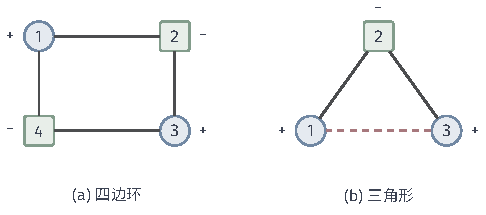
\includegraphics{figures/03-graphs/05-matrices-and-spectra/tikz/incidence-bipartite-signs/figure.pdf}
  \caption{沿环交替分配行符号。圆形顶点保留原行，方形顶点对应的行变号。四边环的每条边都连接异号端点，三角形的虚线边连接两个同号端点。}
  \label{fig:incidence-bipartite-signs}
\end{BookInlineFigure}

\subsection{整数最优解的存在}
\label{sec:incidence-integral-optima}

求最大流时，我们在每个顶点核对流入和流出。求匹配时，在每个顶点数一数选中了几条边。两类问题都是给每条边设一个变量，再用关联矩阵把变量汇总到顶点。如果允许变量取分数值，问题就变成一个普通的线性规划。什么条件能保证放宽后的问题仍有一个整数最优方案？

\subsubsection{关联约束的线性规划}
\label{sec:incidence-lp-models}

把边变量排成向量$\bm{x}$。等式可以规定每个顶点的净流出量，不等式可以限制每条边的容量或每个顶点选边的总量。将等式系数记为$\bm{P}$，上界约束的系数记为$\bm{Q}$，线性松弛可以写成
\begin{equation}
\begin{aligned}
\max_{\bm{x}}\quad &\bm{c}^\top\bm{x}\\
\text{满足}\quad &\bm{P}\bm{x}=\bm{b},\quad
\bm{Q}\bm{x}\leq\bm{d},\quad \bm{x}\geq\bm{0}.
\end{aligned}
\label{eq:incidence-lp-relaxation}
\end{equation}
这里$\bm{b}$和$\bm{d}$是整数数据，$\bm{c}$是目标系数。整数性成立的条件是：把$\bm{P}$和$\bm{Q}$纵向叠在一起得到的矩阵全幺模，并且两个右端都是整数向量。

对每条上界约束，引入一个\term{松弛变量}，记录它还剩多少余量：$\bm{z}=\bm{d}-\bm{Q}\bm{x}\geq\bm{0}$。原来的不等式就等价于$\bm{Q}\bm{x}+\bm{z}=\bm{d}$。把两组等式合在一起，标准型的约束变为
\begin{equation}
\begin{pmatrix}
\bm{P}&\bm{0}\\
\bm{Q}&\bm{I}
\end{pmatrix}
\begin{pmatrix}\bm{x}\\\bm{z}\end{pmatrix}
=
\begin{pmatrix}\bm{b}\\\bm{d}\end{pmatrix},
\qquad \bm{x},\bm{z}\geq\bm{0}.
\label{eq:incidence-lp-slack-matrix}
\end{equation}
每个$\bm{x}$唯一确定一组$\bm{z}$，目标仍为$\bm{c}^\top\bm{x}$。

标准型的系数矩阵右侧多了一个单位阵。看它的任意方子式：如果选中了某个松弛变量的列，这一列在方阵里要么全为零（行列式为零），要么只有一个$1$（沿之展开，阶数降低一）。把选中的松弛列逐一消去，最后剩下的是$\bm{P}$和$\bm{Q}$叠成的矩阵中的一个方子式。如果所有列都是松弛列，消去后空矩阵的行列式按约定等于$1$。因此标准型系数矩阵仍全幺模，右端也仍是整数。

\subsubsection{整数顶点定理}
\label{sec:incidence-integral-vertex-theorem}

把式~\eqref{eq:incidence-lp-slack-matrix}中的原变量和松弛变量合在一起记为$\bm{y}$，右端记为$\bm{r}$，目标系数记为$\bm{a}$（松弛变量的目标系数为零）。标准型变成
\begin{equation}
\max_{\bm{y}}\ \bm{a}^\top\bm{y}
\qquad
\text{满足}\quad \bm{A}\bm{y}=\bm{r},\quad \bm{y}\geq\bm{0}.
\label{eq:incidence-lp-standard}
\end{equation}
线性规划可行且最优值有限时，顶点定理保证最优值能在可行域的某个顶点取得。这里的"顶点"是指不能写成两个不同可行点的凸组合的点。要保证整数最优解存在，只需证明每个顶点的坐标都是整数。顶点定理可参考\BookChapterRef{chap:linear-programming}{卷五"线性规划"章}。

\begin{theorem}[标准型的整数顶点]
\label{thm:graph-tu-integral-vertices}
设式~\eqref{eq:incidence-lp-standard}的系数矩阵$\bm{A}$全幺模，右端$\bm{r}$为整数向量。则可行域的每个顶点都是整数向量。若问题可行且最优值有限，则至少存在一个整数最优解。
\end{theorem}

\begin{proof}
可行域为空时没有顶点需要考察。以下设可行域非空，记$r=\operatorname{rank}\bm{A}$。

先做约化。从$\bm{A}$中选取$r$个线性无关的行，保留对应的右端分量。被删的每一行是所选行的线性组合，把任意可行点代入，可知被删行的右端也是所选右端分量的同一线性组合——因此保留的等式已能推出全部等式。约化后的系数矩阵仍全幺模（方子式只会减少），右端仍为整数。以下继续用$\bm{A}$和$\bm{r}$表示约化后的数据。

若$r=0$，等式约束为空，可行域是$\{\bm{y}\geq\bm{0}\}$。其中每个非零可行点至少有一个正坐标$y_j>0$，沿第$j$个方向正反各动一小步就能把它写成两个不同可行点的中点，所以它不是顶点。只有零向量可能是顶点，它当然是整数向量。以下设$r>0$。

取任意顶点$\bm{y}^\star$，记$S=\{j:y_j^\star>0\}$为正坐标的下标集。我们分三步说明$\bm{y}^\star$为何是整数向量。

第一步：$S$对应的列线性无关。如果相关，就存在非零向量$\bm{h}$，在$S$之外全为零且$\bm{A}\bm{h}=\bm{0}$。取充分小的$\varepsilon>0$使得$\bm{y}^\star\pm\varepsilon\bm{h}$的$S$内坐标仍正，$S$外坐标仍为零。这两个不同的可行点以$\bm{y}^\star$为中点，与顶点定义矛盾。

第二步：将$S$的列补成一组基。$S$对应的独立列数$|S|\leq r$，补选一些列使下标集扩充为$r$列的$J$，令$\bm{A}_J$可逆。$J\setminus S$中的坐标及$J$之外的坐标全为零，因此
\[
\bm{A}_J\bm{y}^\star_J=\bm{r},\qquad \bm{y}^\star_{J^c}=\bm{0}.
\]
$\bm{A}_J$称为\term{基矩阵}，$\bm{y}^\star$是这组基给出的\term{基本可行解}。

第三步：用克莱姆法则求解。$\bm{A}_J$是全幺模矩阵的可逆方形子矩阵，行列式只能为$\pm1$。令$\bm{A}_J^{(i)}$为将$\bm{A}_J$的第$i$列换成$\bm{r}$后的矩阵，克莱姆法则给出
\[
(\bm{y}^\star_J)_i=\frac{\det(\bm{A}_J^{(i)})}{\det(\bm{A}_J)}.
\]
分子是整数矩阵的行列式，本身为整数。分母为$\pm1$。因此每个基坐标都是整数。非基坐标全为零，也是整数。

最后，可行且最优值有限时，由顶点定理取一个最优顶点，它已被证明为整数向量。
\end{proof}

从基矩阵的逆也能看到整数性。由求逆公式，
\[
\bm{A}_J^{-1}=\frac{\operatorname{adj}(\bm{A}_J)}{\det(\bm{A}_J)}.
\]
伴随矩阵$\operatorname{adj}(\bm{A}_J)$的每个条目是一个低一阶的方子式乘以符号，全幺模性保证它们属于$\{0,1,-1\}$。分母为$\pm1$，所以$\bm{A}_J^{-1}$是整数矩阵。用它乘整数右端$\bm{r}$，自然得到整数基坐标。

\subsubsection{图上的整数解}
\label{sec:incidence-integrality-applications}

回到图上的两类问题，分别检查它们的系数矩阵是否满足全幺模条件。

在流量问题里，每个顶点的守恒等式由带符号关联矩阵$\bm{B}$给出，每条弧的容量上界由单位行给出。把$\bm{B}$和$\bm{I}$纵向叠在一起后，任意方子式要么完全来自$\bm{B}$的行列，要么通过沿单位行展开后降阶仍落到$\bm{B}$的子式中。因此堆叠后的矩阵仍全幺模。

在二部匹配问题里，每个顶点的选边额度由无符号关联矩阵$\bm{N}$给出约束$\bm{N}\bm{x}\leq\bm{1}$。每条边恰好连接两个受限的顶点，所以每个$x_e$都被约束在$[0,1]$内。二部图的$\bm{N}$本身已经全幺模（定理~\ref{thm:graph-unsigned-incidence-tu}），松弛变量的单位列不改变全幺模性。

两类问题的右端都是整数，变量都有上界使可行域有界。定理~\ref{thm:graph-tu-integral-vertices}保证只要问题可行，就存在整数最优解。对匹配来说，整数边变量只能取$0$或$1$：$1$表示选中这条边，$0$表示不选。

最大流的流值$F$本身也是变量。图~\ref{fig:incidence-flow-integer-example}展示了一种处理方式：添加一条回流弧$t\to s$，使回流弧的流量$q_4$等于原网络的流值。加上回流弧后，每个顶点（包括源和汇）的守恒式都取零右端。目标就是最大化回流弧上的流量。删去回流弧就还原原图中的流。图中的三点网络里，中转路线$s\to a\to t$受容量$1$限制，直达路线$s\to t$的容量也是$1$，两条各运一个单位，达到最大流值$2$。如果是给定整数供需的最小费用流，则直接以指定的净流出量作为右端。

\begin{BookInlineFigure}
\centering
\begin{tikzpicture}[
  x=1.16cm, y=1cm,
  point/.style={circle,draw=incFlowBlue,fill=incFlowLight,
    minimum size=6mm,inner sep=0pt,line width=.75pt},
  arc/.style={-{Stealth[length=2.2mm]},draw=incFlowLine,line width=.85pt}
]
\definecolor{incFlowBlue}{HTML}{7188A3}
\definecolor{incFlowLight}{HTML}{E5EAF0}
\definecolor{incFlowLine}{HTML}{4C4D4F}
\definecolor{incFlowGreen}{HTML}{829C8B}
\node[point] (s) at (0,0) {$s$};
\node[point] (a) at (2,1.13) {$a$};
\node[point] (t) at (4,0) {$t$};
\draw[arc] (s) -- node[above left] {$q_1\;(2)$} (a);
\draw[arc] (a) -- node[above right] {$q_2\;(1)$} (t);
\draw[arc] (s) -- node[above] {$q_3\;(1)$} (t);
\draw[arc,draw=incFlowGreen,dashed] (t) to[bend left=26]
  node[below] {$q_4\;(3)$} (s);
\end{tikzpicture}

\caption{三点最大流网络。实线标出三条原有弧，括号内是容量。虚线是为守恒记账加上的回流弧，其流量$q_4$等于原网络的流值。}
\label{fig:incidence-flow-integer-example}
\end{BookInlineFigure}

图~\ref{fig:incidence-matching-comparison}对照了全幺模条件成立和失效时的选边方案。

在四边环上，两个交替选边的整数方案各选两条不相邻的边，总量为$2$。四条边各取$1/2$是这两个方案的平均，也达到最优值$2$。这说明整数最优解与分数最优点可以并存。

在三角形上，每条边取$1/2$恰好用满三个顶点的额度，总量为$3/2$。把三个约束$x_{12}+x_{23}\leq1$、$x_{12}+x_{13}\leq1$、$x_{23}+x_{13}\leq1$相加并除以$2$，可知$3/2$已经是松弛问题的上界。而整数匹配最多选一条边，最优值只有$1$。这个间隙的来源正是三角形的无符号关联矩阵行列式为$2$——克莱姆法则中的除法产生了$1/2$。

\begin{BookInlineFigure}
  \centering
  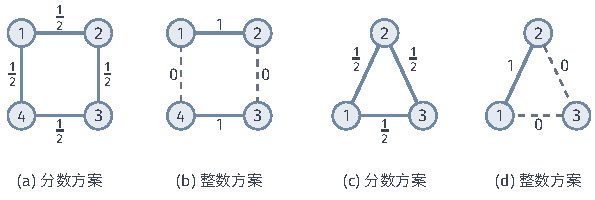
\includegraphics{figures/03-graphs/05-matrices-and-spectra/tikz/incidence-matching-comparison/figure.pdf}
  \caption{四边环和三角形上的选边方案。每个顶点周围的选边量之和都不超过$1$。边旁的数是选边量，实线表示该量为正，虚线表示为零。(a)、(b) 的总量均为$2$，(c)、(d) 分别为$3/2$和$1$。}
  \label{fig:incidence-matching-comparison}
\end{BookInlineFigure}

具体的求解方法见第~\ref{chap:max-flow-min-cut}章、第~\ref{chap:min-cost-flow}章和第~\ref{chap:bipartite-matching-assignment}章。
\section{本章小结}
\label{sec:graph-incidence-summary}

给定参考方向后，图的带符号关联矩阵$\bm{B}\in\mathbb{R}^{n\times m}$在第$e$列（对应有向边$e\colon u\to v$）于尾端$u$记$+1$、头端$v$记$-1$，把顶点函数空间$\mathbb{R}^V$与边空间$\mathbb{R}^E$连接成一对伴随映射：转置矩阵$\bm{B}^\top\colon\mathbb{R}^V\to\mathbb{R}^E$将顶点函数$\bm{f}$映射为沿边差分向量$\bm{d}=\bm{B}^\top\bm{f}$，矩阵本身$\bm{B}\colon\mathbb{R}^E\to\mathbb{R}^V$将边流量向量$\bm{q}$映射为各顶点的净流出向量$\bm{B}\bm{q}$，二者满足伴随恒等式$\langle\bm{B}^\top\bm{f},\bm{q}\rangle_E=\langle\bm{f},\bm{B}\bm{q}\rangle_V$。

在边空间$\mathbb{R}^E$中，每个顶点处净流出量均为零的边流量构成环空间$\mathcal{C}(\mathcal{G})=\ker\bm{B}$，能够表示为顶点函数沿边差分向量的边向量构成割空间$\mathcal{D}(\mathcal{G})=\operatorname{im}\bm{B}^\top$。由伴随恒等式，环空间与割空间正交互补，将边空间正交直和分解为$\mathbb{R}^E=\ker\bm{B}\oplus\operatorname{im}\bm{B}^\top$。

若图有$n$个顶点、$m$条边和$c$个连通分量，则$\ker\bm{B}^\top$由$c$个连通分量的指示向量张成且线性无关，维数为$c$；由秩零度定理，关联矩阵的秩与割空间维数均为$n-c$，环空间维数为$m-n+c$。

选定一棵生成森林$F$后，向$F$中逐一添入$m-n+c$条非树边得到环空间的基本环基（在非树边坐标上构成单位阵），从$F$中逐一删去$n-c$条树边得到割空间的基本割基（在树边坐标上构成单位阵）。

在组合优化中，若整数矩阵的任意阶方子式均属于$\{0,1,-1\}$，则称之为全幺模矩阵。在标准型线性规划中，全幺模系数矩阵与整数右端项使可行域的每个可逆基矩阵行列式均为$\pm1$，由克莱姆法则保证所有极点（基本可行解）均为整数向量，当问题可行且最优值有限时，便存在整数最优解。

按约束矩阵类型划分：以带符号关联矩阵$\bm{B}$为约束的有向网络流家族（最小费用流、最大流、最短路），因$\bm{B}$每列恰有一正一负、对任意无自环图恒全幺模，故在整数供需与容量、问题可行且最优值有限时存在整数最优流；最短路的单位流模型还须排除负费用环。

以无符号关联矩阵$\bm{N}$为约束的配对与覆盖家族（最大匹配、指派问题、最小顶点覆盖），因$\bm{N}$每列有两个$+1$、当且仅当图为不含奇环的二部图时全幺模（奇环子矩阵的排列展开给出行列式$1+1=2$），故在二部图上保证存在$\{0,1\}$整数最优解，而在含奇环图上会出现分数极点。

后续章节将频繁使用本章建立的关联矩阵框架。将沿边差分算子$\bm{B}^\top$、非负边权对角矩阵$\bm{C}$与净流出汇总算子$\bm{B}$依次复合，得到顶点空间上的对称半正定算子$\bm{L}=\bm{B}\bm{C}\bm{B}^\top$——这正是第~\ref{chap:graph-laplacian-matrix}章的组合拉普拉斯矩阵，并在第~\ref{chap:graph-electrical-networks}章的电网络方程中把电势差、支路电导与基尔霍夫电流守恒融为一体。

